\appendix
\chapter{User guide}
\section{Recognition system}
The interface of the library is located in two headers: \texttt{ImageAnalyzer.h} and \texttt{Training.h} in the corresponding namespaces \texttt{ImageAnalyzer.h} and \texttt{Training.h}, respectively. 

\subsection{Creation of shape descriptor}
For both the training and for the recognition shape descriptors are required. The shape descriptors have several rules, that need to be followed by the user in their implementation. The intended purpose of the descriptor is to describe a single 2D shape in a $[0,1]^2$ rectangular area. The descriptor is expected to return the exactly same shape every time and all of its methods should return the same values when called with the same parameters. 

It is also required, that all of the shape descriptor methods are thread safe. It is then recommended to design the shape descriptor as a class with a constant inner state. Not following these rules may result in an unexpected and dysfunctional behavior of the system. 

The user can create a shape descriptor by including the \texttt{ImageAnalyzer.h} header file and inheriting from the class \texttt{ShapeDescriptor}. This class contains several abstract methods, that should be implemented:
\begin{description}
\item[\texttt{GetName()}] Returns the name of the shape a string. This is only for debugging purposes and it does not have to be unique or even constant. However, it is recommended to return a constant unique name among the descriptors.

\item[\texttt{GetPoint(\texttt{float} t)}] Function overload with one parameter \texttt{t} should return a point on the contour of the shape, based on the \texttt{t} parameter. It is recommended to normalize the parameter into $[0,1]$ range by \texttt{NormalizeParam} function.

\item[\texttt{GetPoint(float last\_t, float t, float \& point)}] Function overload with three parameters, that allows the descriptor to describe noncontinuous curves. The \emph{point} parameter passed by a reference should be filled with the same value as from \texttt{GetPoint(t)} as it describes the point of the curve. Then the function should return true if the curve is continuous on the interval $[last\_t, t]$, otherwise false.

\item[\texttt{GetPointsOfInterest()}] Function, that describes places, where an embedded shape may appear. It returns a vector of \texttt{float3} type, where the first two numbers denote the top left corner of the square area, and the third number is the size of the square. It is important for the correct functionality that the points of interest do not overlap with the shape curve, and that they are substantially smaller than the parent shape.
\end{description}

Examples of shapes descriptors can be found in the \texttt{ExampleShapeDescriptors.h} file. Be careful to return the points only in the normalized range $[0,1]^2$.

\subsection{Algorithm properties}
\label{sec:properties}
There are several variables then can be set up and influence the functionality of the software. They can be found in the \texttt{ImageAnalyzer} namespace. Some of them are used both in the training and in the recognition. It is necessary then for the user to be consistent and use the same settings for the recognition as they used for the training.

\begin{description}
\item[\texttt{DEBUG\_IMAGE\_SAVE}] Boolean variable with default value false. Only for debugging purposes. If true, the images created during the recognition are saved as BMP files onto the hard disk into folder \texttt{debug/}, but only in the initial rotation of the image.

\item[\texttt{COMPOSED\_SHAPES\_ENABLED}] Boolean variable with default value true. If false, recognition algorithm recognizes the whole shape but does not search for the pattern shape that might compose it. During training, the generating algorithm does not produce compositions of the shape, so the network is not trained to recognize the composed shapes.

\item[\texttt{COMPOSITION\_SAMPLES\_COUNT}] Integer variable describing the amount of samples taken when searching for the pattern shapes. This variable has no effect when composed shapes are disabled. Otherwise, the interval $[0,1]$ is sampled uniformly and each sample is passed into the \texttt{GetPoint} method of the descriptor. The returned point is then expanded into the sampling window and checked for pattern shape.

\item[\texttt{COMPOSITION\_WINDOW\_SIZE}] Float variable that describes the size of the sampling window used during pattern shape matching. The actual window is a square with a side size of 2*\texttt{COMPOSITION\_WINDOW\_SIZE}. This variable has no effect when composed shapes are disabled.

\item[\texttt{COMPOSITION\_SAMPLES\_LIMIT}] Integer variable describing the number of minimum pattern shape matches. If the count of the pattern shape matches is lower, the pattern shape is not recognized. This variable has no effect when composed shapes are disabled.

\item[\texttt{EMBEDDED\_SHAPES\_ENABLED}] Boolean variable with default value true. If false, recognition algorithm ignores the \texttt{GetPointsOfInterest} method of the shape descriptor, where embedded shapes might be, and recognizes only the top level shape and its composing shape. During training, the generating algorithm will not generate embedded shapes, and the network will not be trained to filter out these locations, where the embeddings could appear.

\item[\texttt{ROTATIONS\_ENABLED}] Boolean variable with default value true. If false, recognition algorithm will not test different shape rotations for the best match, but will use the initial rotation. This variable does not have an impact on training since rotation recognition is not a direct task of the neural network.

\item[\texttt{ROTATION\_SAMPLES\_COUNT}] The amount of samples created when matching rotated shape. It directly determines the rotation step angle size, which is in degrees 360/\texttt{ROTATION\_SAMPLES\_COUNT}. This variable has no effect when rotations are disabled.

\item[\texttt{DEBUG\_OUPUT}] Integer variable with default value 1. Controls the amount of debug info of the recognition system. If set to 0 or lower, no debug output is produced. If set to value 1, it prints recognized shape with its matching rotation and its composing shape to the standard output, for the top level shape and each embedded shape. If set to 2 or higher, produces the same output as with value 1, but also all network outputs from the analysis are printed for all the rotations.

\item[\texttt{IMAGE\_SIDE\_SIZE}] Integer variable, controls the size of the images that are created anytime during algorithm. Every time there is an instance of \texttt{ImageLines} class that should be analyzed by the network, the lines are drawn into the square pixel map of a size set by this variable and then serialized as an input to the network. The network input layer size has to be the second power of this value. The default value is 32, which means that the neural network has an input layer of size 1024 neurons, and the images produced in the algorithm are pixel maps of $32*32$ pixels.

\end{description}

\subsection{Training phase}
Training the neural network consists of several steps. The first step is to set up the variables controlling the behavior of the recognition and training algorithms. By including the \texttt{Training.h} file, the user can access the \texttt{ImageAnalyzer} namespace for setting up the variables, and the \texttt{Training} namespace for the training functions. 
After setting the variables, it is necessary to register the desired shape descriptors through function the \texttt{Training::RegisterShapeDescriptor}. This function takes a unique pointer to the shape descriptor as its parameter, and returns an instance of the \texttt{ShapeIndex} class. This class is only a wrapper over integers but it works as an identifier of the shape in the algorithm and the calls to the \texttt{ImageAnalyzer::Analyze} will return the \texttt{ShapeIndex} for each recognized shape. 
The next step is to call the \texttt{Training::Train} function. This function has several parameters:
\begin{description}
\item \texttt{std::string name} Describes the name of the neural network. When the network is created and trained, it is saved under the current working directory into the file with the name \texttt{name} with the extension \texttt{.net}.
\item \texttt{vector<unsigned int> networkStructure} This parameter describes the layers of the network. Each number represents number of neurons in a single layer. The first number describes the size of the input layer, while the last number describes the size of the output layer. The user can set any number of layers higher than two, and arbitrary sizes of layers, apart from the first and last layer.  The first layer has to be equal to the second power of \texttt{IMAGE\_SIDE\_SIZE}, and the last layer size has to be equal to the number of registered shape descriptors.
\item \texttt{boolean generateData = true} Parameter that controls whether the training algorithm should generate the training data. The algorithm looks for training data in the current working directory in the file \texttt{training.data} and for test data in file \texttt{test.data}. If the parameter is true, the algorithm will generate these two files, possibly overwriting them. If the parameter is false, the algorithm uses the files found, or ends with error, of the files are not found.
\item \texttt{float targetMSE = 0.01} The MSE that the network should achieve on the \texttt{test.data}. The training stops if the network achieves MSE lower than this value, or if the network does not improve anymore. 
\item \texttt{int dataSize = 300 000} The parameter describing the number of generated training samples in the \texttt{training.data}. The size of the generated test data is one third of this value. if the parameter \texttt{generateData} is false, then this parameter is ignored. 
\end{description}
after the training process finishes, the network is ready to be used in the recognition algorithm.

\subsection{Recognition phase}
When the neural network is ready, the user can set up the recognition system and use it in a game. The recognition system is used through interface located in the \texttt{ImageAnalyzer} namespace in \texttt{ImageAnalyzer.h} file. The namespace contains definition of the algorithm properties, as well as definition for classes that the user is supposed to use, namely the \texttt{ShapeDescriptor} class, the \texttt{ImageLines} class and the \texttt{ShapeIndex} class.

First, it is necessary to load the neural network into the algorithm, using \texttt{ImageAnalyzer::LoadNetwork} function, which takes string describing the path to the network as an argument. Then, the user has to register the same descriptors used for the training of the loaded network again, but this time using the \texttt{ImageAnalyzer::RegisterShapeDescriptor}, which takes the corresponding \texttt{ShapeIndex} instance together with the descriptor.

Alternatively, the \texttt{ShapeIndex} instance can be created from the order number of the corresponding shape descriptor when registered for the training. It is also necessary to set up the algorithm properties the same way they have been set up during network training. When these steps are done, the user can repeatedly call the \texttt{ImageAnalyzer::Analyze} function to determine the shape hierarchy in the provided \texttt{ImageLines} instance. The \texttt{Analyze} function is thread safe, so many calls can be done at the same time. However, the set up has to be done synchronously and only once, before the first call of \texttt{Analyze} function. 

\section{Game}
The game is a simple prototype. When the game is started the character controlled by player is located in the middle of the screen. The character can move over the surface plane, but falling of the edge results in death. There will be also numerous enemies around. initially, all the enemies are harmless and the player has control over the AI activity. This feature was added because it was too difficult to draw more complicated spells without dying. The goal of the game is to destroy all the enemies, either trough usage of totems or character's attacks.

\subsection{Controls}
The game uses both keyboard and mouse with the following mappings:
\begin{itemize}
\item[W, A, S, D] The player can control the character using the keys W,A,S,D to move the character up, left, down and right respectively.
\item[E, R] The keys E and R can be used to turn off, respectively on, the AI of the enemies.
\item[Q] Using the Q key and pointing the mouse over the enemy, the players character starts moving towards the enemy and attacking it.
\item[Left mouse button] The player can draw shapes on the ground using the left mouse button.
\item[Right mouse button] By pushing the right mouse button, the player invokes spell casting.
\item[Mouse wheel] Mouse wheel can be used to zoom in/zoom out.
\end{itemize}

\subsection{Spells}
The spells in the game are represented by totems. When the player casts a spell, a totem is created with corresponding effects on it, described by the rules below.
The game supports four shapes: circle, square, triangle and water drop. Each of these shapes maps to a different effect, based on its position in the drawing. We distinguish between 3 positions of shapes: the root position, the embedded shape and the pattern shape.
\begin{itemize}
\item The root position is assigned to the biggest shape, i.e. the shape that forms the drawing. 
\item The embedded shape is a shape that is located in the center of another shape. 
\item The pattern shape is a shape that forms a composition of another shape.
\end{itemize}
Relations between the shape position, shape and effect are described by the following rules:
\begin{description}
	\item The root shape mappings: 
	\begin{itemize}
		\item[Circle] The \emph{Shield} effect \ref{fig:spell:circle} is added to the totem. If the players character is inside the area of effect of this totem, its shield is slowly recharged.
		\item[Square] The \emph{Fire} effect \ref{fig:spell:square} is added to the totem. The fire effect causes all enemies near the totem to burn, decreasing their health periodically.
		\item[Triangle] The \emph{Freezing} \ref{fig:spell:triangle} effect is added to the totem. The freezing effect causes the enemies to move slowly.
		\item[Water drop] The \emph{Healing} \ref{fig:spell:waterDrop} effect is added to the totem. When the players character is nearby, it is healed over time.
	\end{itemize}
	\item The embedded shape mappings:
	\begin{itemize}
		\item[Circle] The \emph{Reach} effect \ref{fig:spell:embcircle} is added to the totem, extending its area of effect twice.
		\item[Square] The \emph{Power} effect \ref{fig:spell:embsquare} is added to the totem. The power effect causes all the attacks of the player do substantially more damage to the enemies.
		\item[Triangle] The \emph{Durability} effect is added to the totem. The durability effect extends the duration of the totem twice.
		\item[Water drop] The \emph{Distraction} effect \ref{fig:spell:embwaterDrop} is added to the totem. Enemies under the distraction effect start attacking the totem instead of the player.
	\end{itemize}
	\item The pattern shape mappings:
	\begin{itemize}
		\item[Circle] The \emph{DefenseWall} effect \ref{fig:spell:patcircle} is added to the totem. When the totem with the defense wall is created, it creates a wall around it.
		\item[Square] The \emph{Explosions} effect \ref{fig:spell:patsquare} is added to the totem. This effect causes the enemies to explode, slowing them and reducing their health.
		\item[Triangle] The \emph{Tower} effect \ref{fig:spell:pattriangle} is added to the totem. The totem with the tower effect starts shooting at any enemy that appears in its area of effect.
		\item[Water drop] The \emph{Madness} effect is added to the totem. Enemies under the madness effect start attacking randomly each other.\footnote {While this effect is supported in theory, in reality since it the pattern shape is always classified as an circle rather than a water drop, due to the imperfections of the algorithm.}
	\end{itemize}
\end{description}

\begin{figure}[p]
\centering
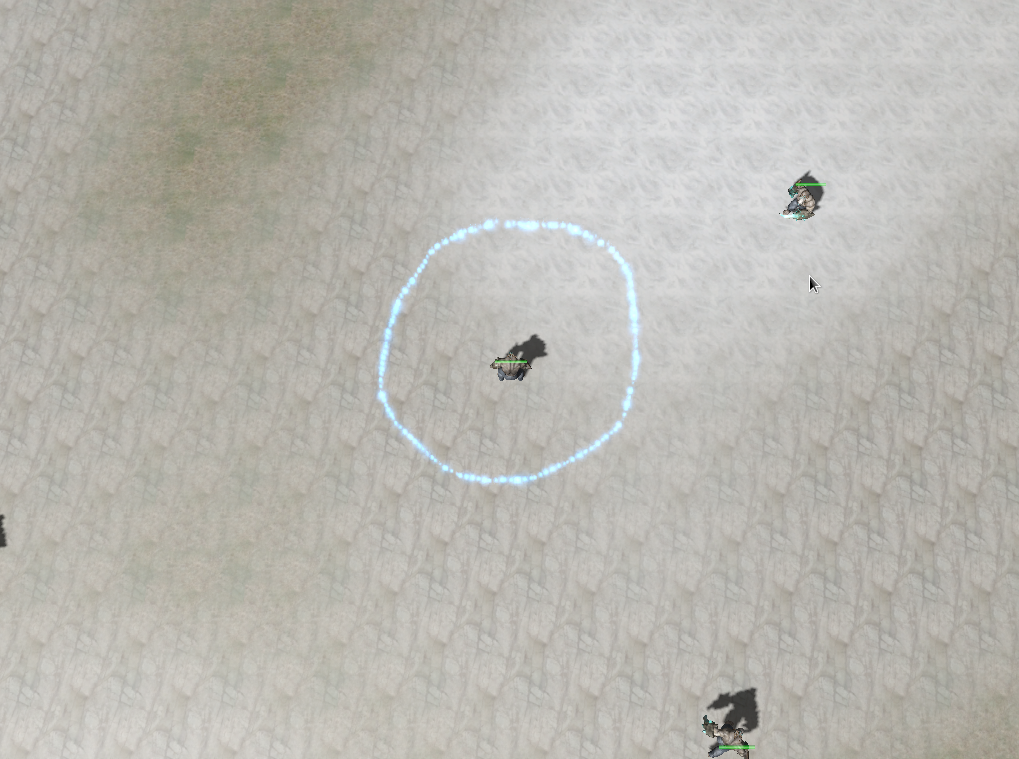
\includegraphics[width=.9\linewidth]{ext/scr/circle.png}
\quad
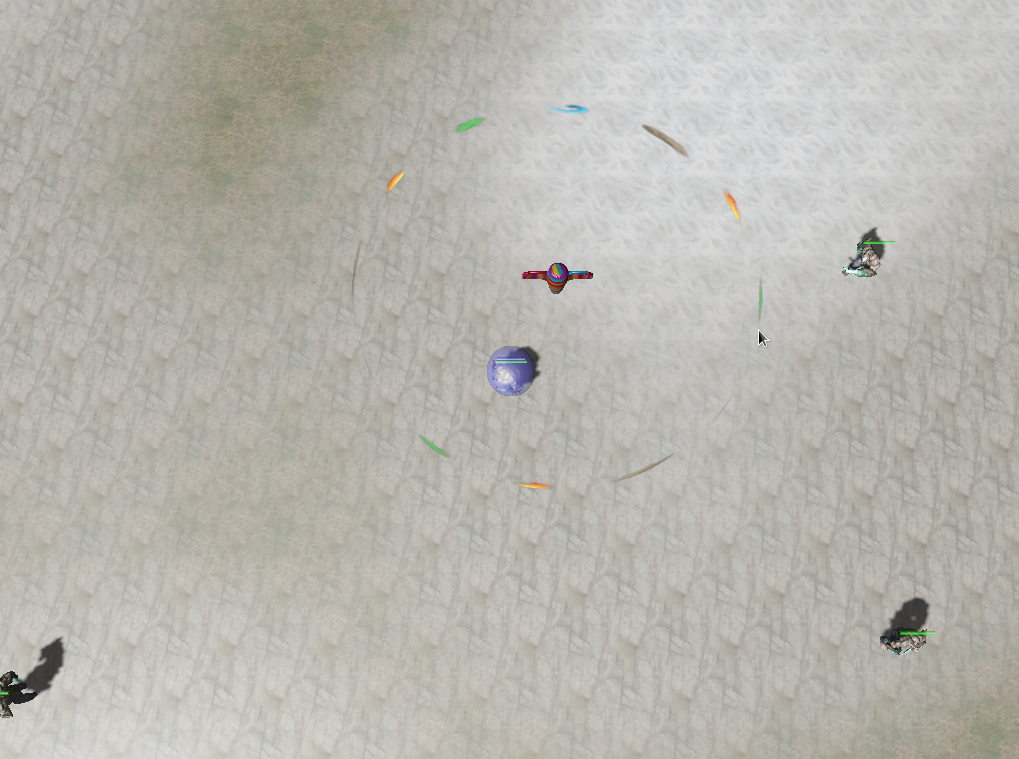
\includegraphics[width=.9\linewidth]{ext/scr/circlee.png}
\caption{The figures show a drawn circle and the created \emph{Shield} effect totem. The player's character has a shield recharging on it. }
\label{fig:spell:circle}
\end{figure}

\begin{figure}[p]
\centering
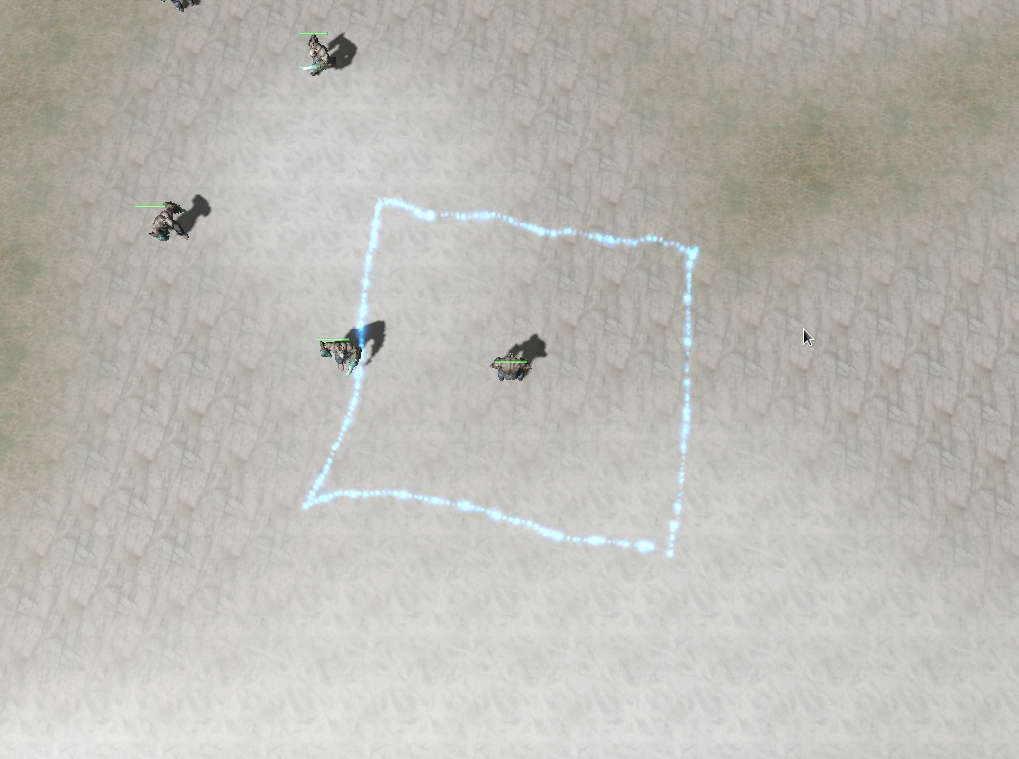
\includegraphics[width=.9\linewidth]{ext/scr/square.png}
\quad
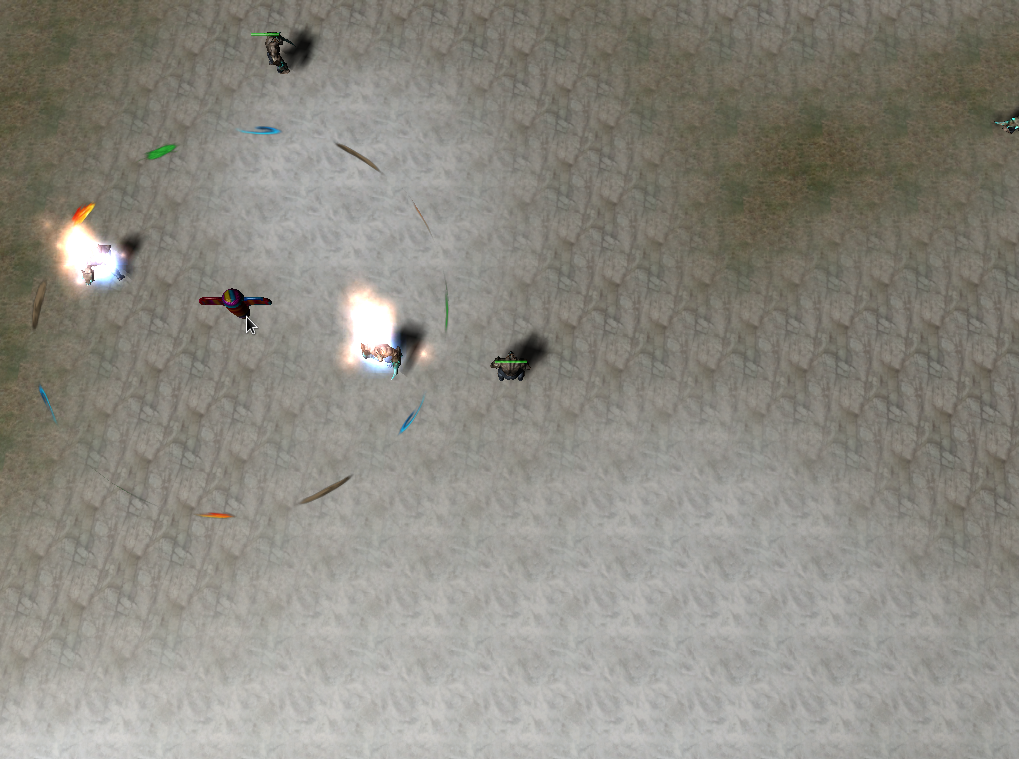
\includegraphics[width=.9\linewidth]{ext/scr/squaree.png}
\caption{The figures show a drawn square and the created \emph{Fire} effect totem. The enemies in the area of effect of the totem are burning. }
\label{fig:spell:square}
\end{figure}

\begin{figure}[p]
\centering
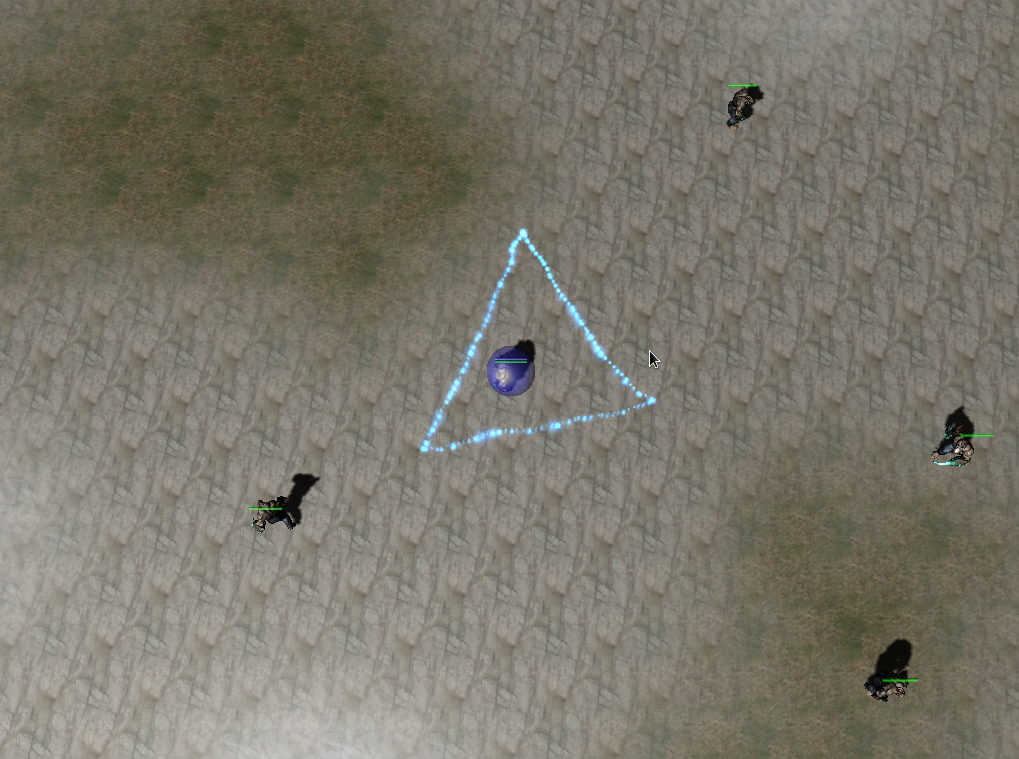
\includegraphics[width=.9\linewidth]{ext/scr/triangle.png}
\quad
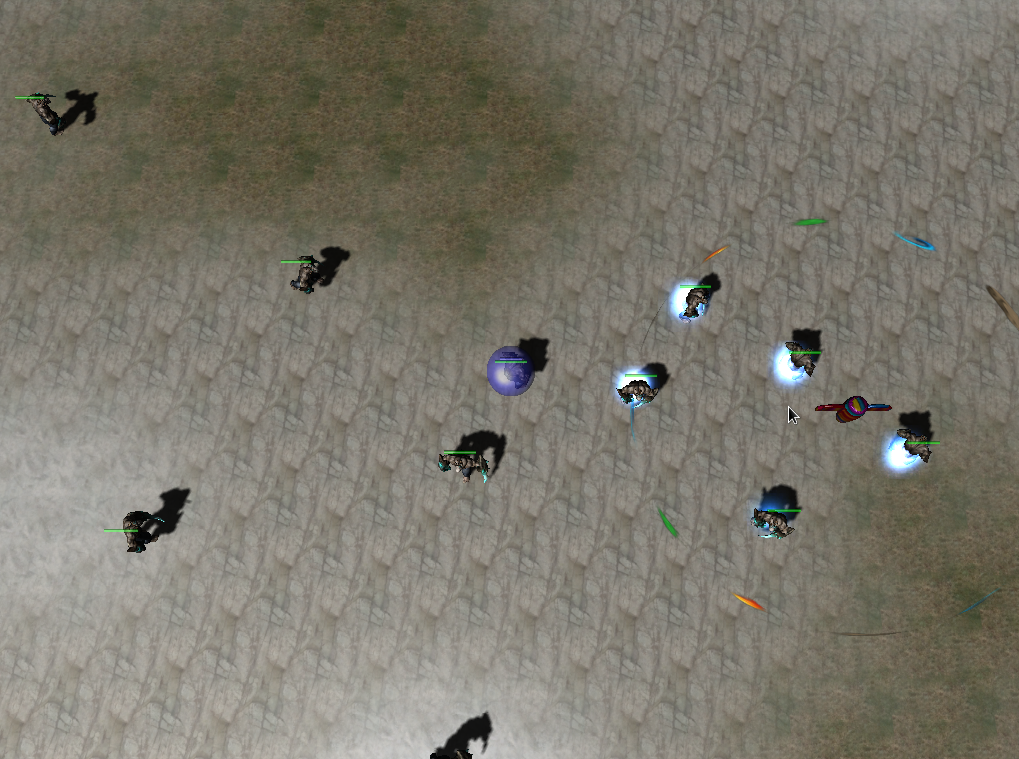
\includegraphics[width=.9\linewidth]{ext/scr/trianglee.png}
\caption{The figures show a drawn triangle and the created \emph{Freezing} effect totem. The enemies in the area of effect of the totem are slower.}
\label{fig:spell:triangle}
\end{figure}

\begin{figure}[p]
\centering
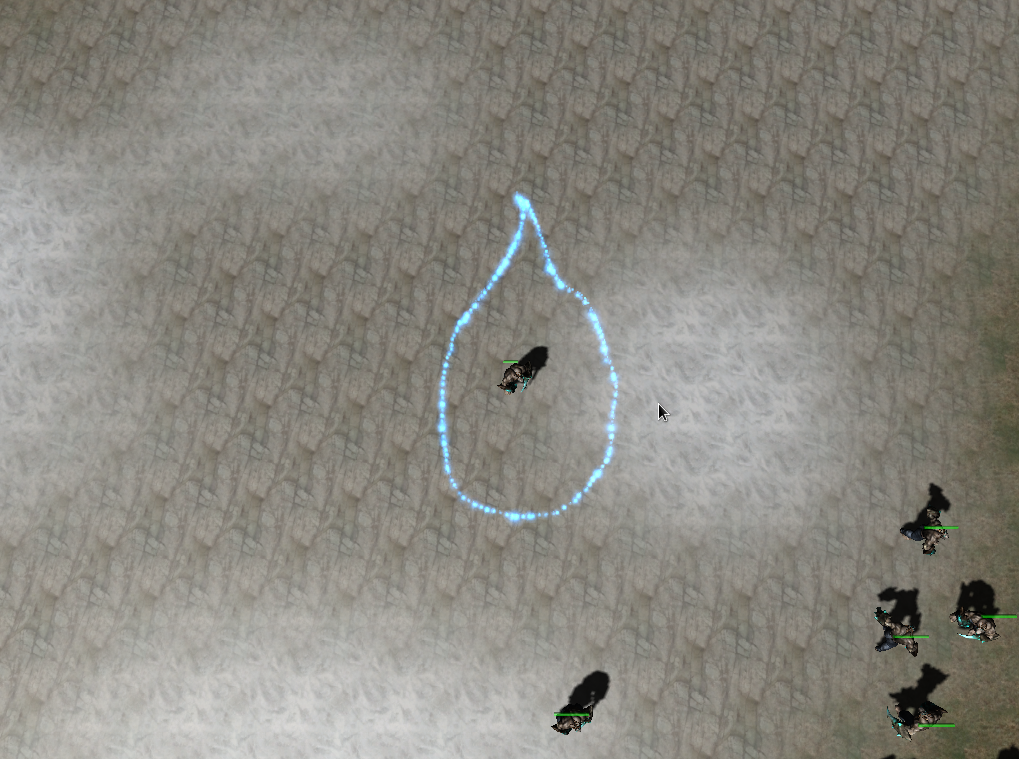
\includegraphics[width=.9\linewidth]{ext/scr/waterDrop.png}
\quad
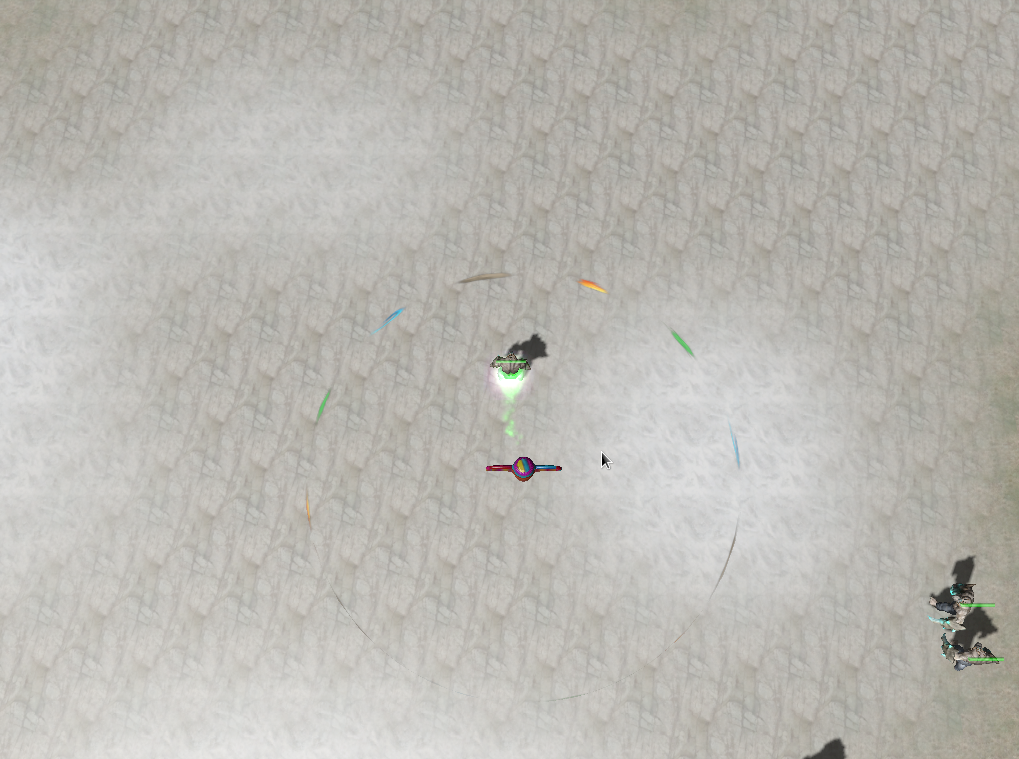
\includegraphics[width=.9\linewidth]{ext/scr/waterDrope.png}
\caption{The figures show a drawn water drop and the created \emph{Healing} effect totem. The player's character is healed in the presence of the totem.}
\label{fig:spell:waterDrop}
\end{figure}

\begin{figure}[p]
\centering
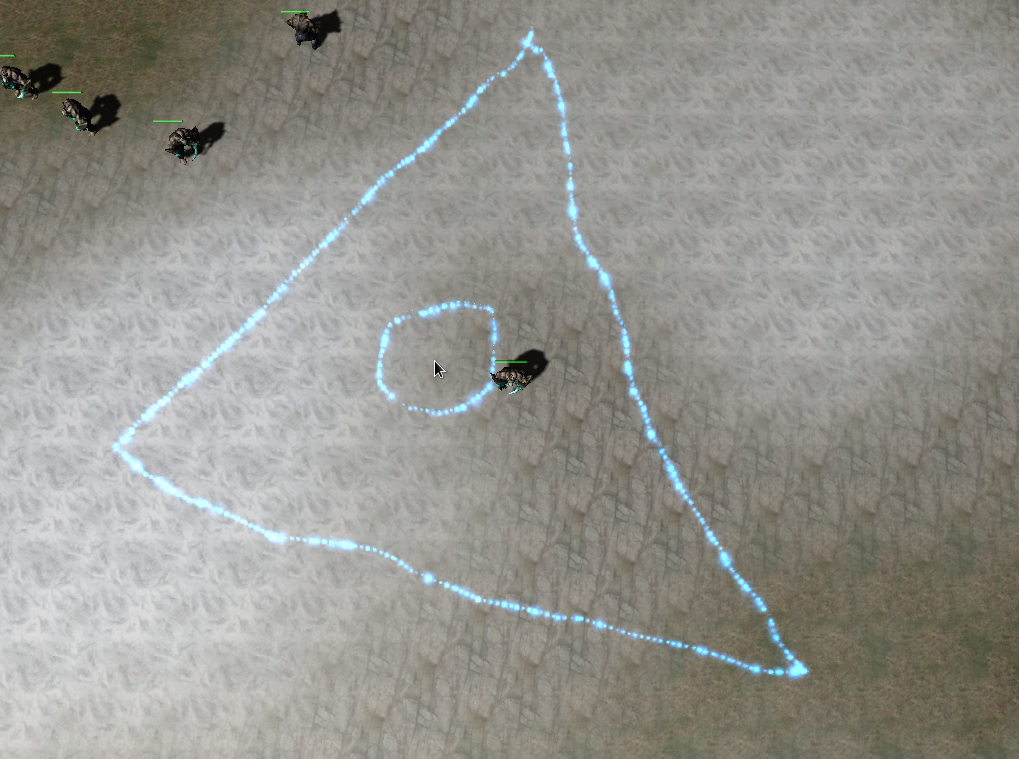
\includegraphics[width=.9\linewidth]{ext/scr/embcircle.png}
\quad
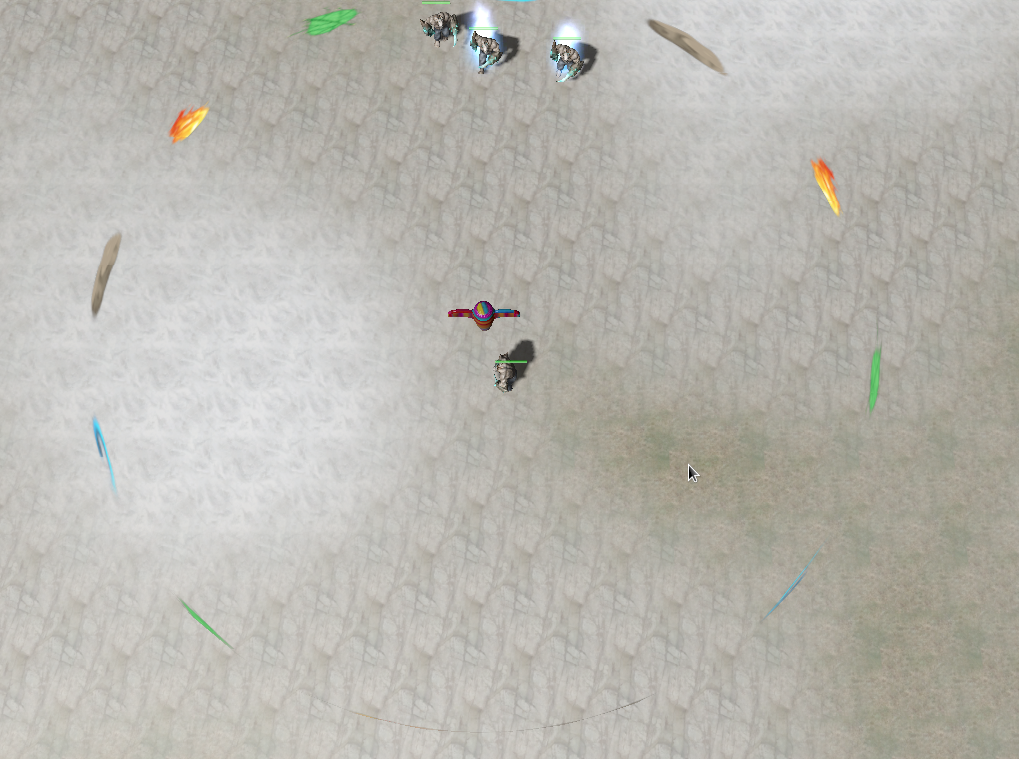
\includegraphics[width=.9\linewidth]{ext/scr/embcirclee.png}
\caption{The first figure shows a triangle with an embedded circle. The second figure shows the created totem has the are of effect increased twice. }
\label{fig:spell:embcircle}
\end{figure}

\begin{figure}[p]
\centering
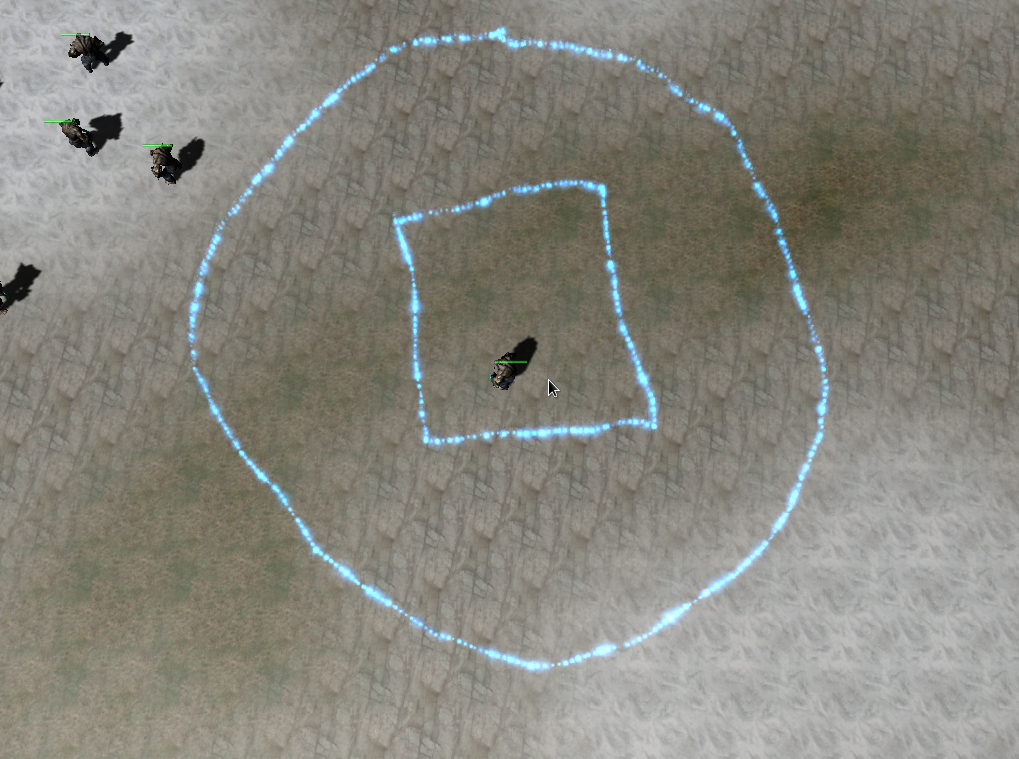
\includegraphics[width=.9\linewidth]{ext/scr/embsquare.png}
\quad
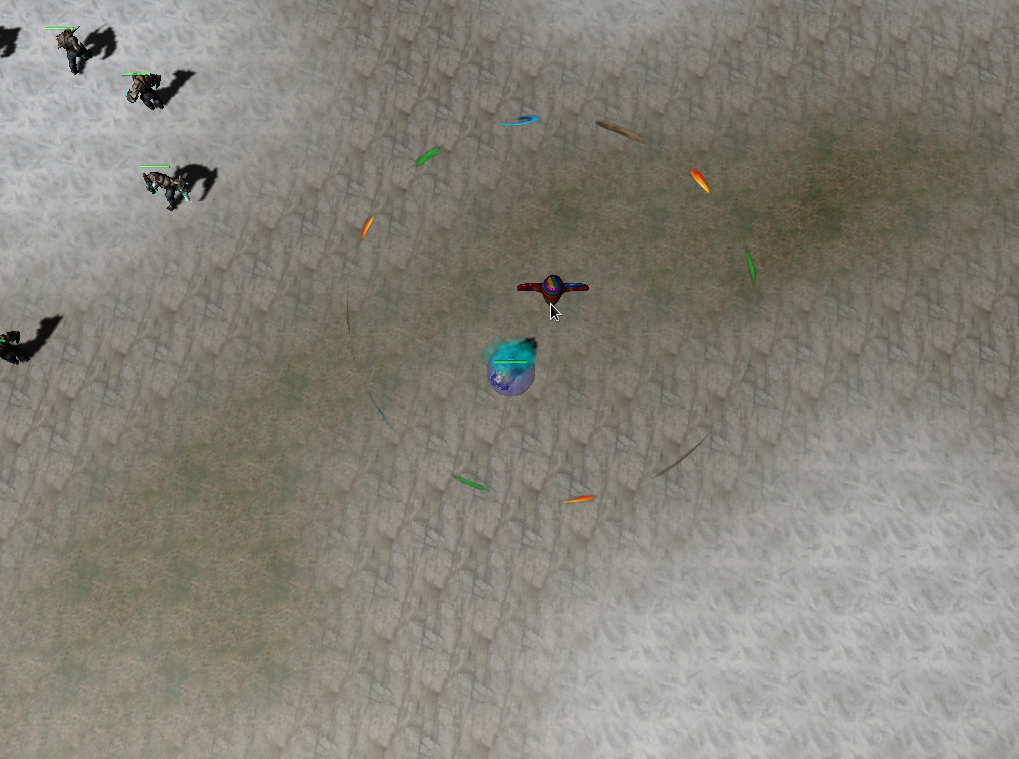
\includegraphics[width=.9\linewidth]{ext/scr/embsquaree.png}
\caption{The first figure shows a circle with an embedded square. The second figure shows the created totem shields the character and grants it power state, increasing its attack.}
\label{fig:spell:embsquare}
\end{figure}

\begin{figure}[p]
\centering
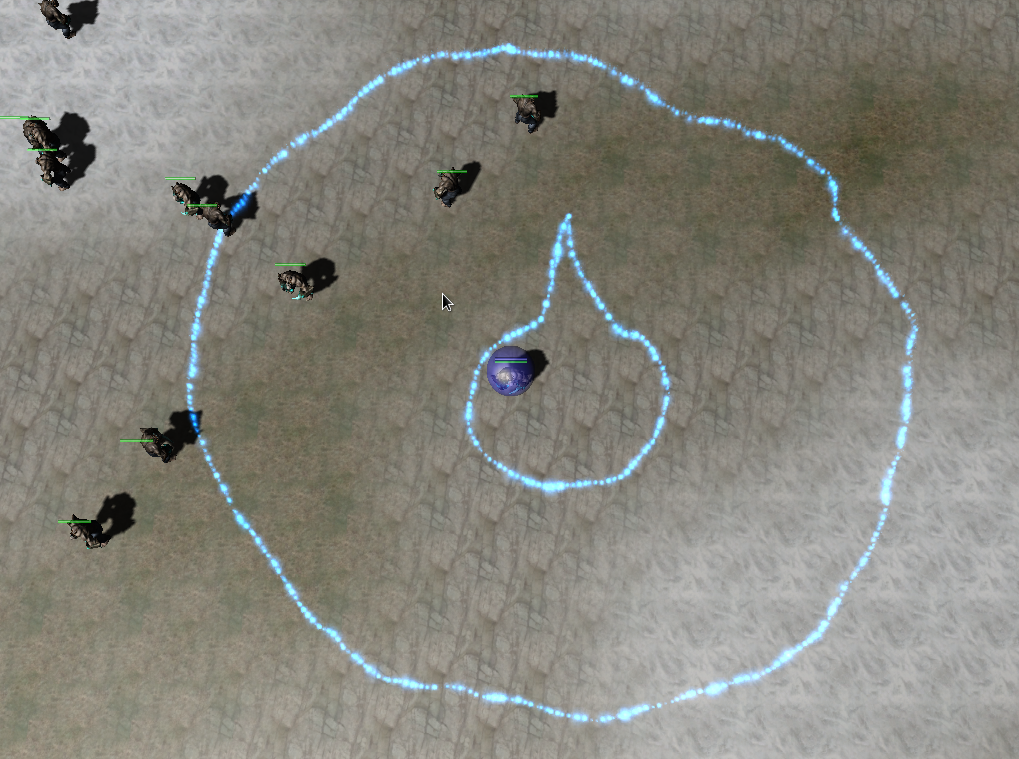
\includegraphics[width=.9\linewidth]{ext/scr/embwaterDrop.png}
\quad
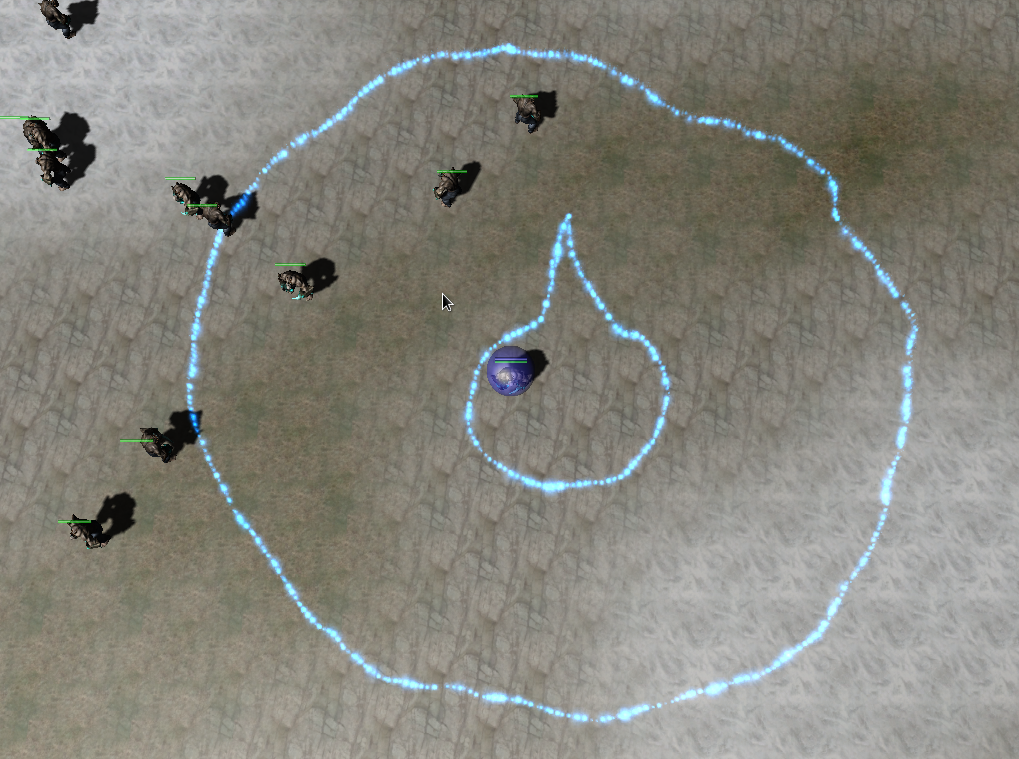
\includegraphics[width=.9\linewidth]{ext/scr/embwaterDrop.png}
\caption{The first figure shows a circle with an embedded water drop. The second figure shows the created totem shields the character and its \emph{Distraction} effect lures the enemies.}
\label{fig:spell:embwaterDrop}
\end{figure}


\begin{figure}[p]
\centering
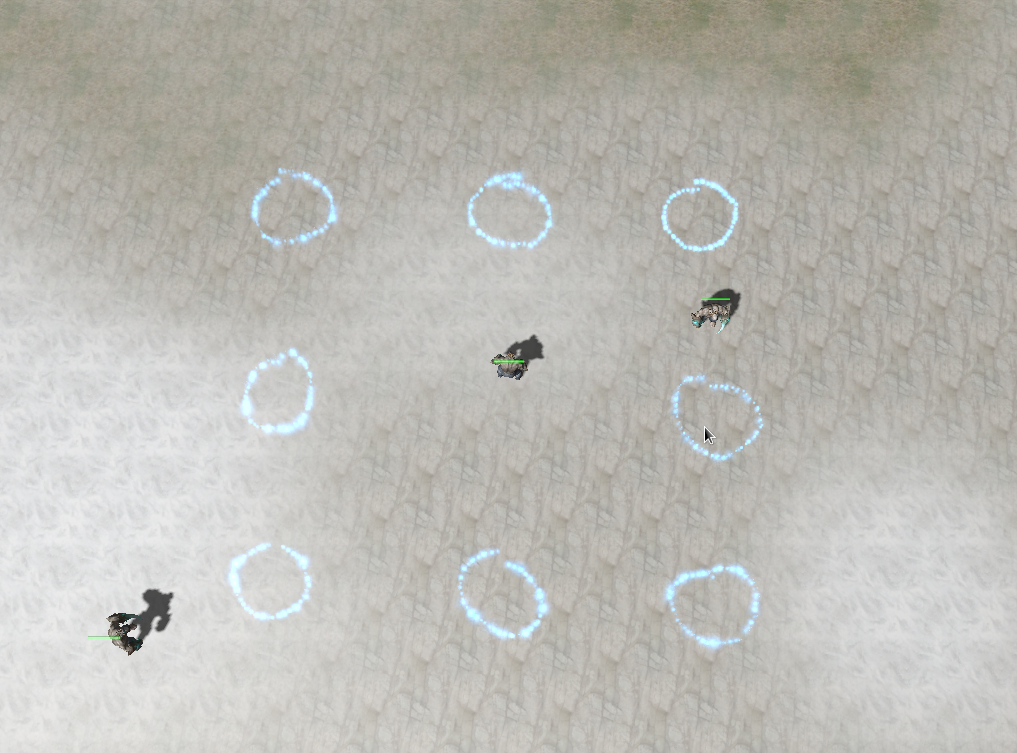
\includegraphics[width=.9\linewidth]{ext/scr/patcircle.png}
\quad
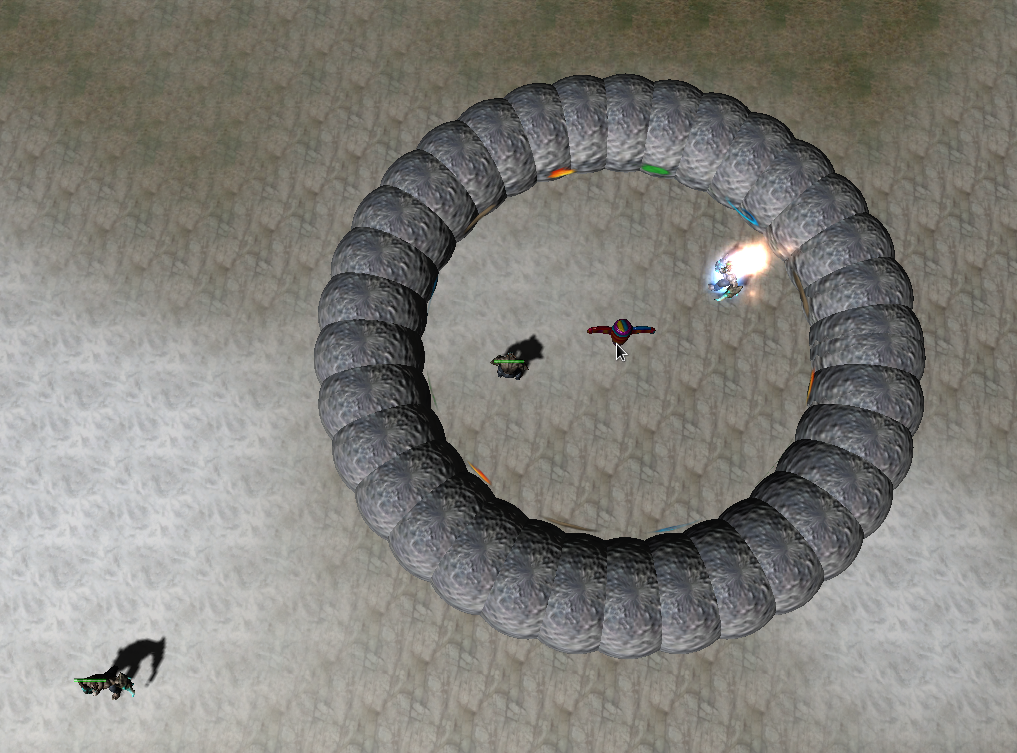
\includegraphics[width=.9\linewidth]{ext/scr/patcirclee.png}
\caption{The first figure shows a square composed from circle pattern shapes. The second figure shows the \emph{WallEffect} caused by the circle pattern shape. }
\label{fig:spell:patcircle}
\end{figure}

\begin{figure}[p]
\centering
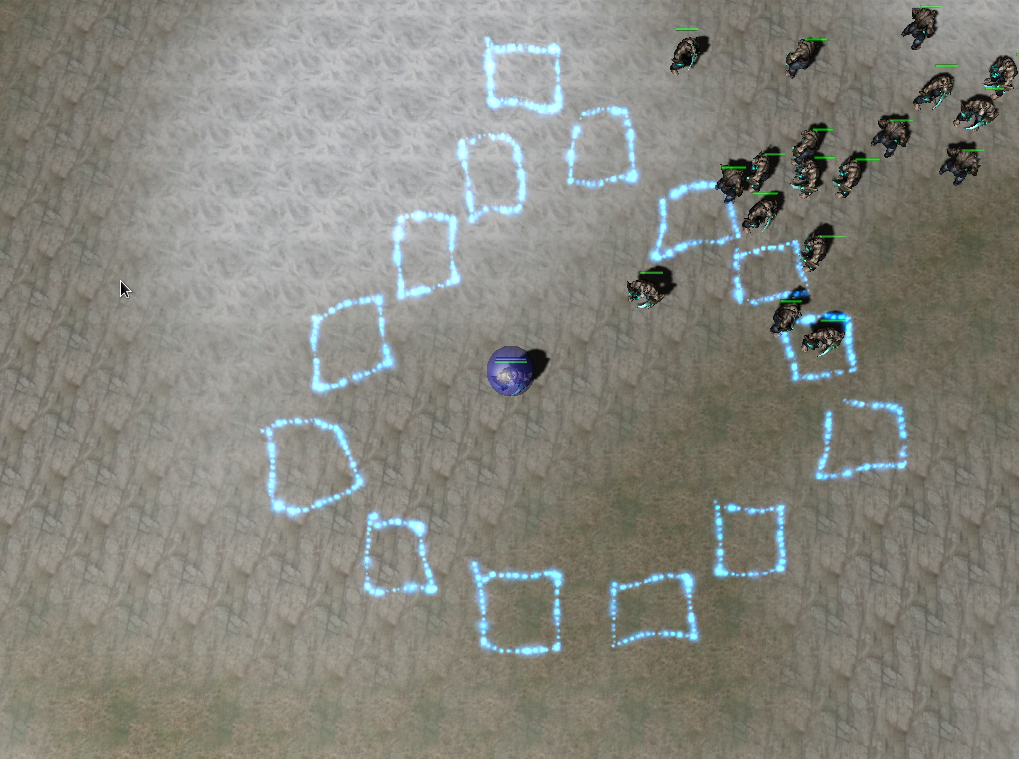
\includegraphics[width=.9\linewidth]{ext/scr/patsquare.png}
\quad
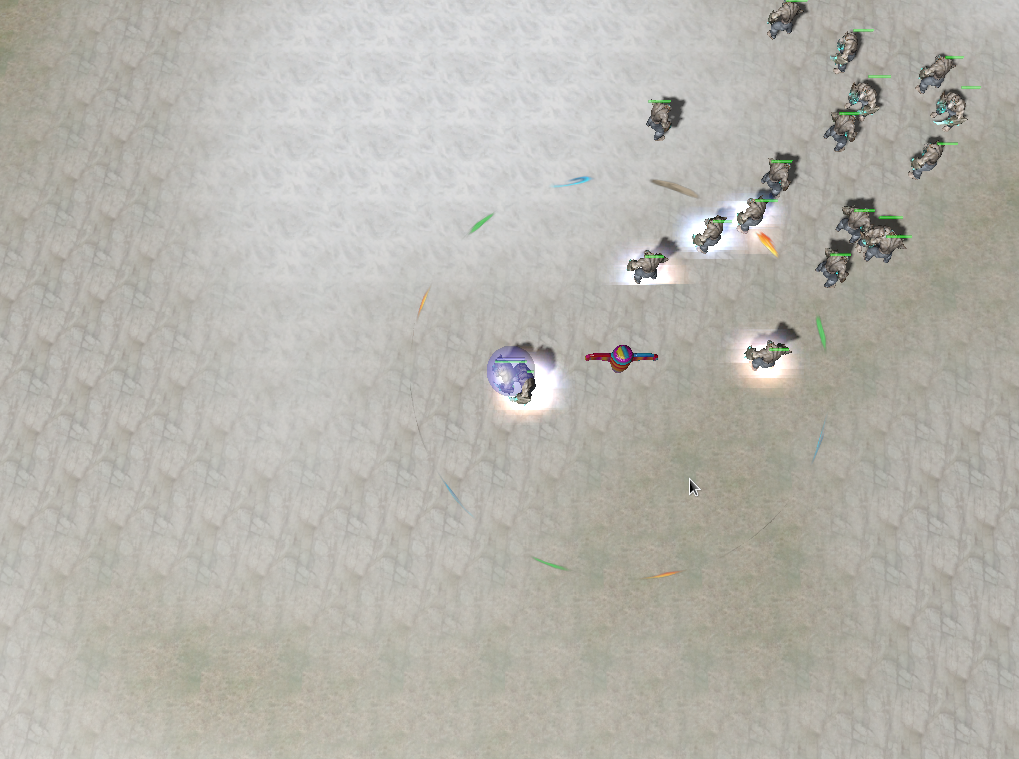
\includegraphics[width=.9\linewidth]{ext/scr/patsquaree.png}
\caption{The first figure shows a water drop composed from square pattern shapes. The second figure shows an explosions effect caused by the square pattern shape. }
\label{fig:spell:patsquare}
\end{figure}

\begin{figure}[p]
\centering
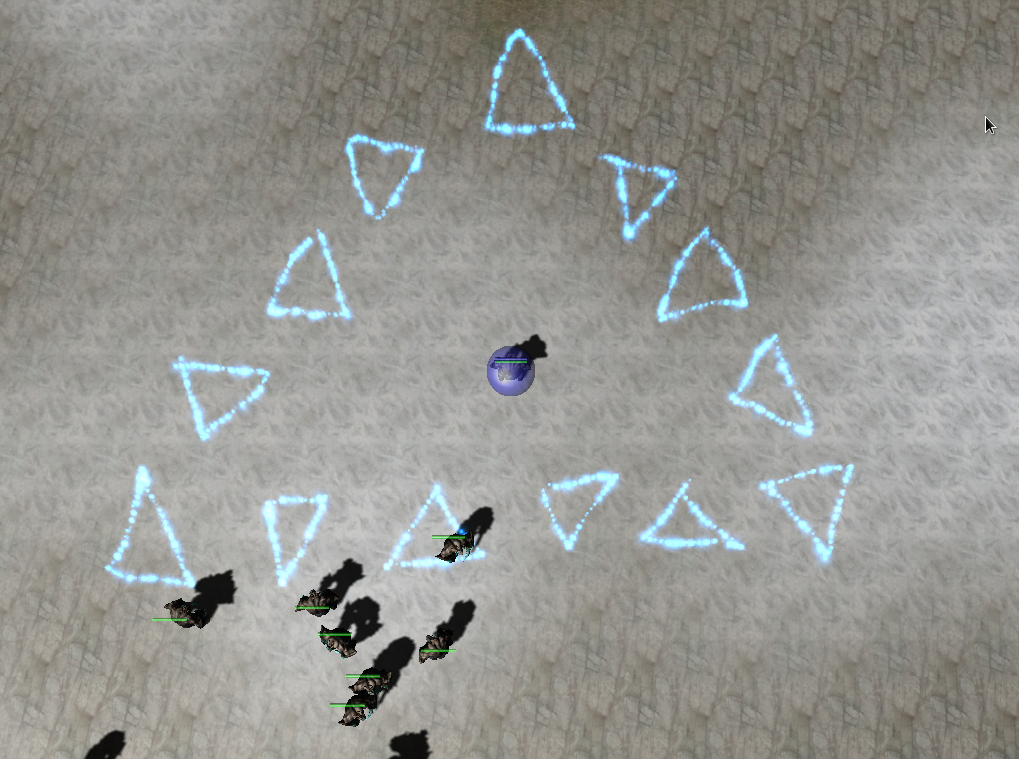
\includegraphics[width=.9\linewidth]{ext/scr/pattriangle.png}
\quad
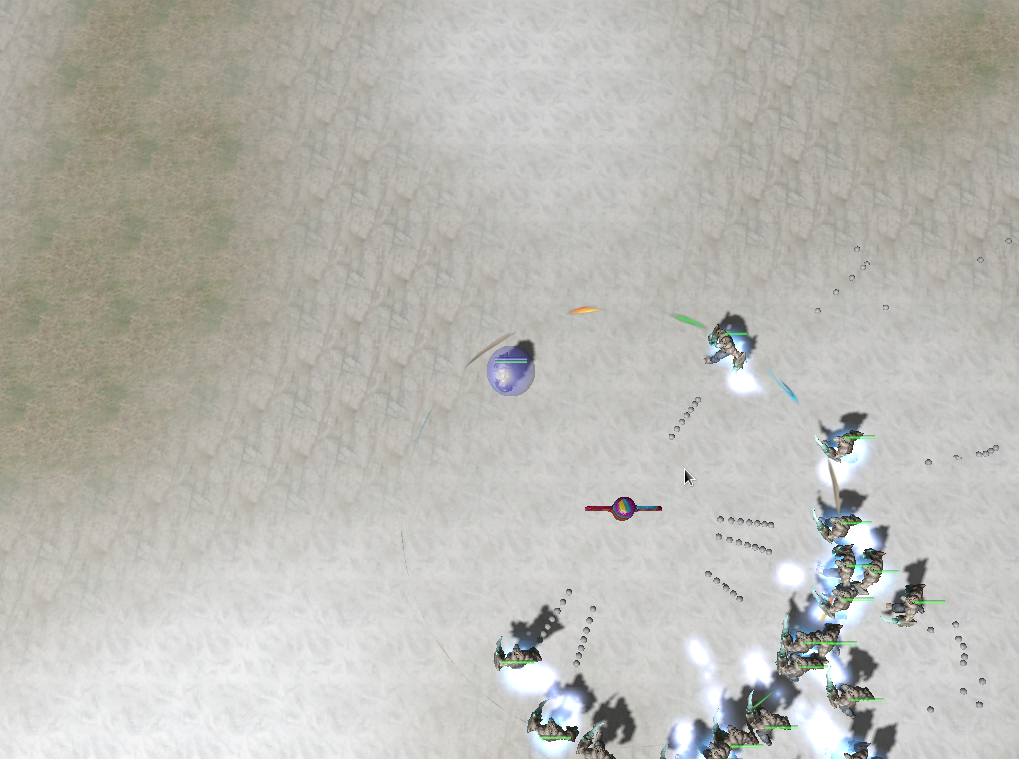
\includegraphics[width=.9\linewidth]{ext/scr/pattrianglee.png}
\caption{The first figure shows a triangle composed from triangle pattern shapes. The second figure shows the \emph{Tower} effect caused by the triangle pattern shape. }
\label{fig:spell:pattriangle}
\end{figure}

